\begin{figure}[h]
\centering
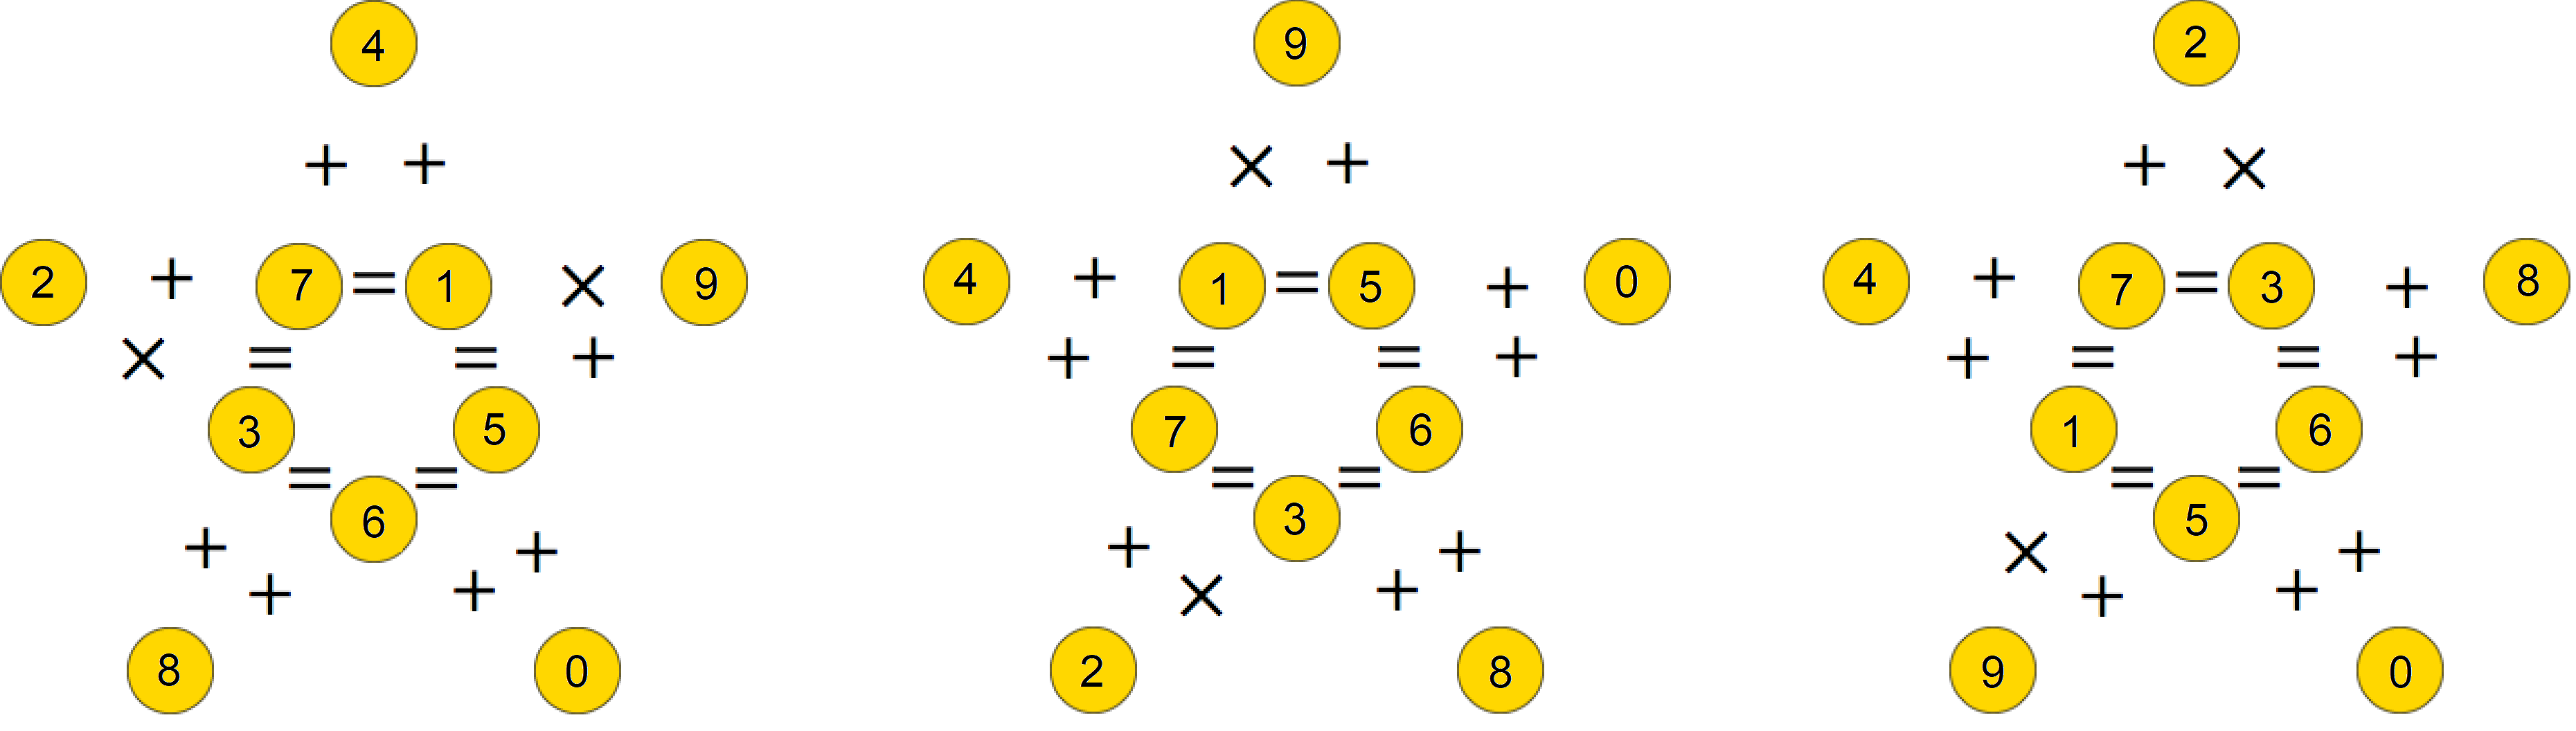
\includegraphics[width=\textwidth]{figuras/rotated.png}
\caption{A estrela do centro tem a configuração [3,1,1,1,1,1,3,1,1,1]. A estrela da esquerda é obtida através de uma rotação da estrela do centro, formando a configuração [1,1,3,1,1,1,1,1,3,1]. A estrela da direita é obtida através de uma combinação de uma rotação e uma reflexão, resultando na configuração [1,3,1,1,1,1,1,3,1,1]}
\label{fig: ops_restriction}
\end{figure}